\documentclass[10pt,a4paper]{report}
\usepackage[utf8]{inputenc}
\usepackage[english]{babel}
\usepackage[T1]{fontenc}
\usepackage{amsmath}
\usepackage{amsfonts}
\usepackage{graphicx}
\usepackage{lmodern}
\usepackage{amssymb}
\usepackage{verbatim}
\usepackage{float}
\usepackage{minitoc}
\usepackage{amsthm}
\newtheorem{definition}{Definição}
\newtheorem{theorem}{Teorema}
\usepackage{hyperref}
\title{\LARGE{Network and Computer Security } \\ \vspace{0.5cm} \normalsize{Summary}}
\date{}

\begin{document}
\maketitle
\tableofcontents

\chapter{Cryptography}
It is a widespread and dangerous belief that encrypting everything provides protection against anything. In reality, when the algorithm is known it is necessary to prevent several types of attacks, such as ciphertext-only, known-plaintext, chosen-plaintext or chosen-ciphertext. Cryptography must, then, protect the information against unauthorized insertion of information, modification of information in transit, replay of information and access to information.
\section{Cryptographic Services}
To this end, we need the following cryptographic services:
\begin{itemize}
\item Confidentiality: a service used to keep the content of the information from all, but those entities authorized to have it. Has the drawbacks of making debugging harder and may lead to information loss if the key is lost. Can be assured through symmetric of assymetric cipher.
\item Integrity: a service that detects data manipulation by unauthorized entities (not the same thing as error detection codes). An intruder should not be able to substitute a false message for a legitimate one. Can be assured through MIC or a digital signature.
\item Authenticity: a service used to ascertain the identity or the origin of a message. Can be assured through MIC or a digital signature, tough freshness requires adding a nonce to the message.
\begin{itemize}
\item Entity authentication: verify the identity of an entity
\item Data origin authentication: confirm the creator of the message
\item Non-repudiation: a service which prevents an entity from denying. Can be assured by a digital signature.
previous commitments or actions
\end{itemize}
\end{itemize}
\section{Cryptographic Building Blocks}
\subsection{Symmetric Cipher}
Uses the same key to cipher and decipher. In cryptographic function notation:
\begin{itemize}
\item $E(M,K)$: cipher message $M$ with key $K$
\item $D(C,K)$: decipher cryptogram $C$ with key $K$
\end{itemize}
\subsection{Asymmetric Cipher}
A public/private pair of keys is used ($KU/KR$). In cryptographic function notation:
\begin{itemize}
\item $AE(M, KR)$: cipher message $M$ with private key $KR$
\item $AD(C, KU)$: decipher cryptogram $C$ with public key $KU$
\end{itemize}
It is also possible to cipher with the public key and then decipher with the private key.
\subsection{Cryptographic Hash}
A cryptographic hash function does not use a key, instead receives an input message and returns a digest of the data. In cryptographic function notation:
\begin{itemize}
\item $H(M)$: hash of message $M$
\end{itemize}
The digest value is deterministic, has fixed size, a unique representation, is non-reversible and sensible to input changes.
\subsection{Composite Building Blocks}
\begin{itemize}
\item Hybrid cipher: a random symmetric key is generated and used to cipher the message. This key is then ciphered with the public key of the receiver and is sent along with the ciphered message. The receiver must decipher the symmetric key with its private key and use it do decipher the message
\item Message integrity code: the MIC is created by creating the digest of the message and ciphering the result. It can then be used to check the integrity of the message by generating a new hash and comparing to the sent one.
\item Digital signature: a digital signature is created by ciphering a digest with the private key. The receiver can then decipher with the public key and verify the identity of the sender.
\end{itemize}
\section{Symmetric Criptography}
Symmetric ciphers use a single secret key that may be shared by 2 or more communicating parties. This allows confidentiality to all those who have the key and message authentication, with good performance. The main problem lies in key distribution\\
\\
For $N$ communicating parties, $N \times (N-1) / 2$ keys are needed for them to be able to communicate 1 - 1 secretly.\\
\\
An example of a symmetric cipher is the one-time pad, where the message is XOR'd with the key. The security is based on the assumption that the key is never reused.
\subsection{Symmetric Stream Ciphers}
Symmetric stream ciphers are pratical approximations to the one-time pad. Keystreams are generated in a deterministic way from a fixed size key (approximation to real random sequence generators).
\begin{figure}[H]
\centering
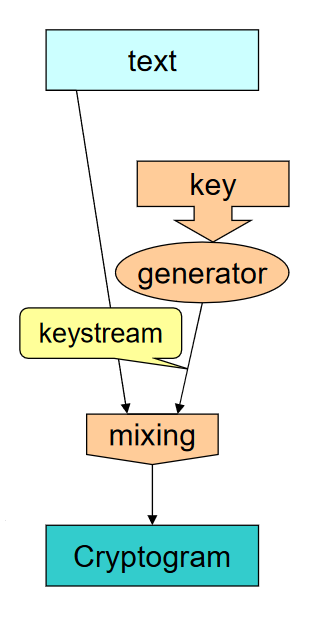
\includegraphics[scale=0.4]{1.png}
\end{figure}
In this type of cipher, if the plain text is known, the keystream is exposed. The secure pseudo-random generators are sometimes based on LFSRs (Linear Feedback Shift Registers). It consists on a state machine that produces a cyclic sequence of bits:
\begin{figure}[H]
\centering
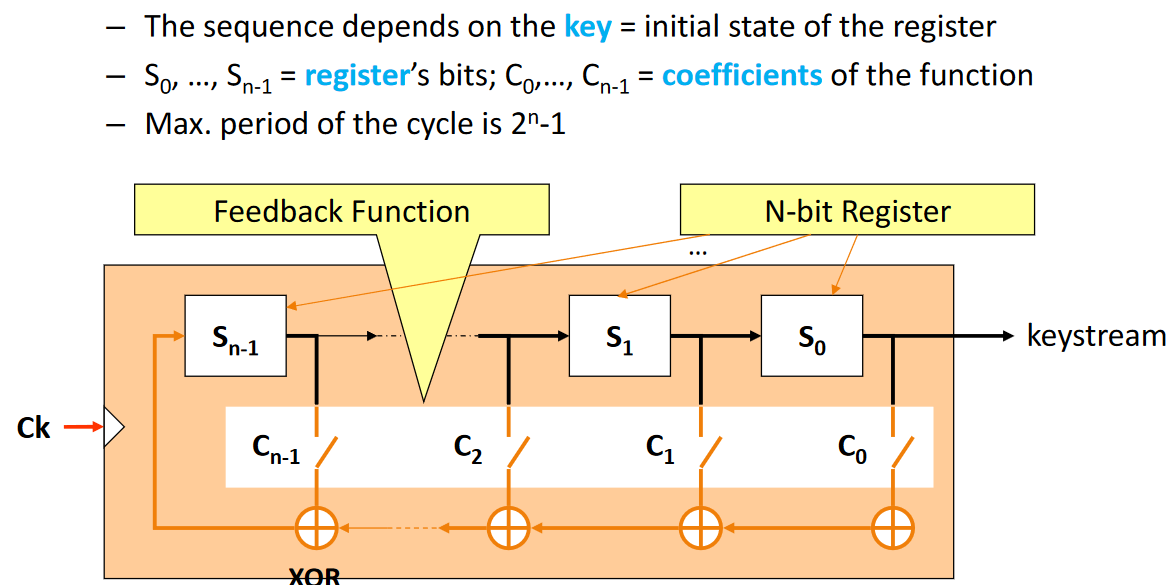
\includegraphics[scale=0.4]{2.png}
\end{figure}
\subsection{Symmetric Block Ciphers}
These are also  based on approximations, using Shannon’s notions of confusion (repeated application of a complex function to a large block) and diffusion (permutation, substitution, expansion and compression).
\subsubsection{Feistel Network}
The feistel network is a complex  function most commonly
used in block cipher algorithms. It applies a round function $F$ over multiple rounds:
\begin{itemize}
\item Each round uses a different round key ($K_i$), obtained from the key ($K$)
\item Text is split in left (L) and right (R) parts
\end{itemize}
The cipher and decipher processes are the same, with the keys used in the inverse order.
\begin{figure}[H]
\centering
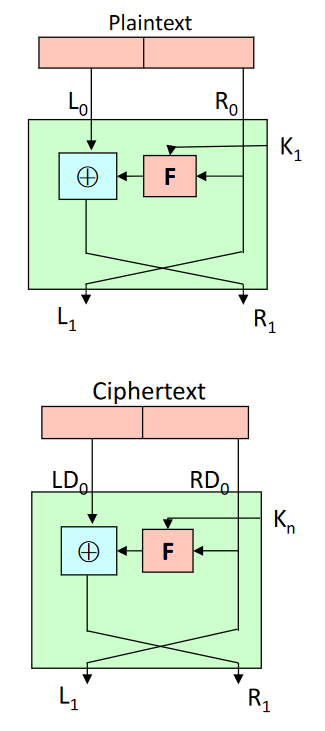
\includegraphics[scale=0.4]{3.png}
\end{figure}
\subsubsection{DES}
The DES algorithm uses 64 bit blocks with 56 bit keys. It applies the feistel network algorithm on several rounds, after an initial permutation of the 64 bits, according to a fixed table.
\subsubsection{Block Cipher Modes}
When using a plaintext of different size than the block, a cipher mode must be used.
\begin{itemize}
\item $Electronic$ $Code$ $Book$ (ECB)
\begin{itemize}
\item Encryption using independent blocks
\item Weakness in reproducing patterns from the original text; identical blocks produce the same ciphertext
\end{itemize}
\begin{figure}[H]
\centering
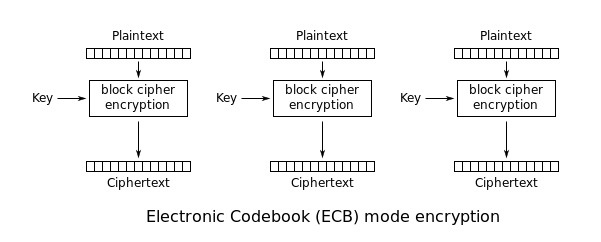
\includegraphics[scale=0.5]{4.png}
\end{figure}
\item $Cipher$ $Block$ $Chaining$ (CBC)
\begin{itemize}
\item Plaintext is XORed with the ciphertext of the previous block before encryption
\item Reduces the risk of pattern replication
\item Uses an initialization vector in the first block (necessary for decryption) and requires padding: bits to compose entire blocks of the size required by the algorithm
\end{itemize}
\begin{figure}[H]
\centering
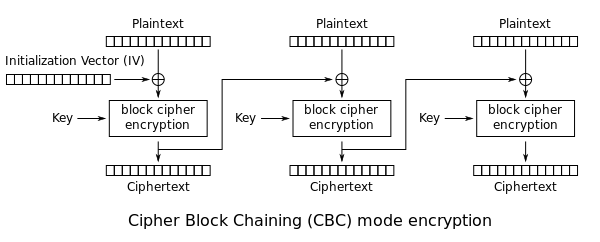
\includegraphics[scale=0.5]{5.png}
\end{figure}
\item $Output$ $Feedback$ (OFB)
\begin{itemize}
\item Retains the advantages of CFB, and the ciphertext is not used in the next block, allowing block cipher operations to be performed in advance, enabling parallel XOR as soon as the text (plaintext or ciphertext) is available
\end{itemize}
\begin{figure}[H]
\centering
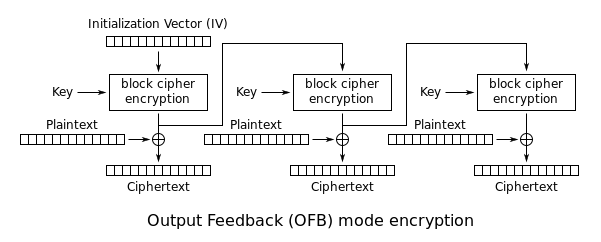
\includegraphics[scale=0.5]{6.png}
\end{figure}
\item $Counter$ $Mode$ (CTR)
\begin{itemize}
\item Standard cipher mode in AES
\item Uses a nonce and a counter, which must be different in each cipher operation
\end{itemize}
\begin{figure}[H]
\centering
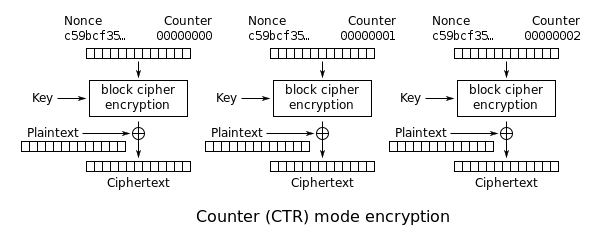
\includegraphics[scale=0.5]{7.png}
\end{figure}
\item $Galois$ $Counter$ $Mode$ (GCM)
\begin{figure} [H]
\centering
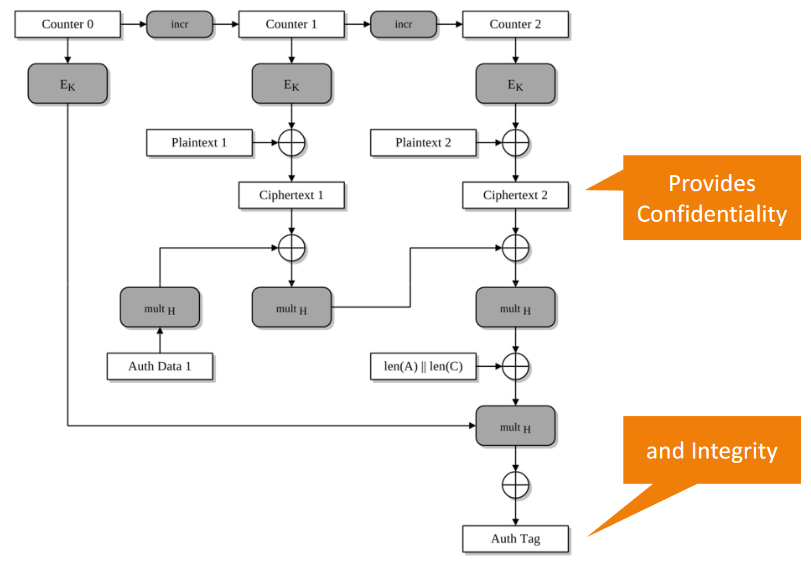
\includegraphics[scale=0.4]{8.png}
\end{figure}
\end{itemize}
\subsubsection{Padding}
Sometimes it may be necessary to pad the last block, when the message size is not divisible by the block length. This may be done by:
\begin{itemize}
\item Padding with zero (null) bytes, spaces (0x20), all bytes of the same value
\item Padding with random bits
\item Padding with 0x80 (1000 0000) followed by zero (null) characters
\item Padding with the PKCS\#5 scheme: Sequence of bytes, each of which equal to the number of padding bytes (e.g.   if 24 bits of padding need to be added, the padding string is "03 03 03": 3 bytes times 8 bits equals 24)
\end{itemize}
\subsubsection{AES}
AES is the current encryption standard. Supports keys of 128, 192 and 256 bits with 128 bit blocks. It runs in 10, 12 or 14 rounds, in which it substitutes bytes, shifts rows, mixes columns and adds the round key XOR state with key material)
\section{Hash Functions}
These are cryptagraphic functions, but not ciphers. They must be:
\begin{itemize}
\item Collision resistance: Computationally infeasible to find two inputs that give the same hash
\item Preimage resistance: Given a hash, it’s computationally infeasible to find an input that produces that hash
\item Seconde preimage resistant: Given a hash value and the corresponding input, it’s computationally infeasible to find a second input that generates that same hash
\end{itemize}
The most common algorithms are:
\begin{itemize}
\item MD5 (128 bits): very weak
\item SHA-1 (160 bits): weak
\item SHA-2 (256 to 512 bits)
\item SHA-3 (256 to 512 bits)
\end{itemize}
Attacks on hash functions are sometimes done by brute force ($P(collision) = 2^{m-1}$) and most often through the birthday attack ( pick $M$, $M'$, $M''$, $M'''$... and obtain hashes until any 2 are identical) ($P(collision) = 2^{m/2}$).
\subsection{Message Integrity Codes}
The objective is to detect changes to a message. It allows the checking of a message's integrity and, with freshness can provide authenticity, thus, it's sometimes called MAC.\\
\\
Under the assumption that the sender and recipient have a shared secret key $K$, the idea is to send the messgae and the MAC; if the message (or the MAC) is modified by an attacker, the recipient will be able to detect it. Attacker cannot create a valid MIC because he does not have $K$.\\
\\
Implementations of MAC could be as follows:
\begin{itemize}
\item Hash the message and encrypt the digest
\item Using a keyed-function (CMAC, usually with CBC)
\item Using a keyed-hash (HMAC)
\end{itemize}
\section{Asymmetric Ciphers}
Asymmetric cryptography uses a pair of public/private keys. It allows for confidentiality, authentication and integrity (digital signatures). Has the advantage of only needing $N$ key pairs, but the performance is much worse.\\
\\
For confidentiality, the public key is used to cipher and the private to decipher. For authentication it's the opposite.
\subsection{One-way Functions}
Also known as trapdoor functions. The idea is for the function to be easy to compute in one direction, but hard to invert. These are usually used in asymmetric cryptography.
\subsection{Algorithms}
\subsubsection{RSA}
In this algorithm, the plaintext is divided into blocks, which are treated as a number. The keys are generated as follows:
\begin{itemize}
\item Choose two prime numbers $p$ and $q$
\item Define $n = pq$ and $z = \phi(n) = (p-1)(q-1)$
\item Choose $e < n$ such that $e$ is coprime with $z$
\item Calculate $d$ such that $ed \mod z = 1$
\item The public key is $K_u = (e, n)$, and the private key is $K_r = (d, n)$
\end{itemize}
To encrypt, compute:
$$
E(K_u, m) = m^e \mod n = c
$$
And to decrypt:
$$
D(K_r, c) = c^d \mod n = m
$$
RSA is often used to produce signatures. To sign $M$ we calculate $S = (hash(M))^d \mod n$ and to verify we check $hash(M) == S^e \mod n$. Only the owner of the private key can sign, but anyone with the public key can verify the signature.
\subsubsection{ECC}
Elliptic curve cryptography offers the same security as RSA with smaller bit sizes. In this case, the "hard" problem is the elliptic curve logarithm:
\begin{itemize}
\item $Q = k \cdot P$, where $Q, P$ belong to an elliptic curve (e.g. $y^2 = x^3 - 3x + b \mod p$)
\item Easy to compute $Q$, given $k$ and $P$
\item Hard to find $k$, given $Q$ and $P$
\item $P$ is a base point (parameter of the curve)
\end{itemize}
\subsection{Digital Signatures}
Digital signatures use an asymmetric cipher and a hash function. The basic algorithm is as follows:
\begin{itemize}
\item Sign: $S(doc) = E(K_r, hash(doc))$
\item Validate: $D(K_u, S(doc)) == hash(doc)$
\end{itemize}
Today often ECDSA is adopted (with elliptic curve encryption).

\section{Public Key Management}
In the past, public keys were distributed by means of public directories or announcements. Currently, the distribution is done through the use of digital certificates.
\subsection{Digital Certificates}
Certificates are documents signed by a certification entity (CA, public organization or company)
\begin{itemize}
\item Public documents
\item Have a digital signature
\item Used to distribute public keys through unsecure channels
\item Contain version, serial number (of the CA), issuer, validity, etc.
\end{itemize}
\subsubsection{Certificate Issuance}
\begin{itemize}
\item Keys to assure confidentiality
\begin{itemize}
\item The public key of $X$ is used by the sender to assure confidentiality of the data sent to $X$
\item The private key of $X$ is used to decipher the received information
\item These keys can be refreshed frequently
\end{itemize}
\item Keys to assure authentication
\begin{itemize}
\item The private key of X is used to sign the content
\item The corresponding public key to validate the signature
\item These keys should not be renewed frequently
\end{itemize}
\end{itemize}
\subsubsection{Certificate Distribution}
There is a PKI (Public Key Infrastructure) to manage certificates in a certain context (e.g. the web). It encompasses a set of CAs (and similar entities), policies and mechanisms, and supports several operations, like the creation of key pairs or distribution of certificates.
\begin{figure}[H]
\centering
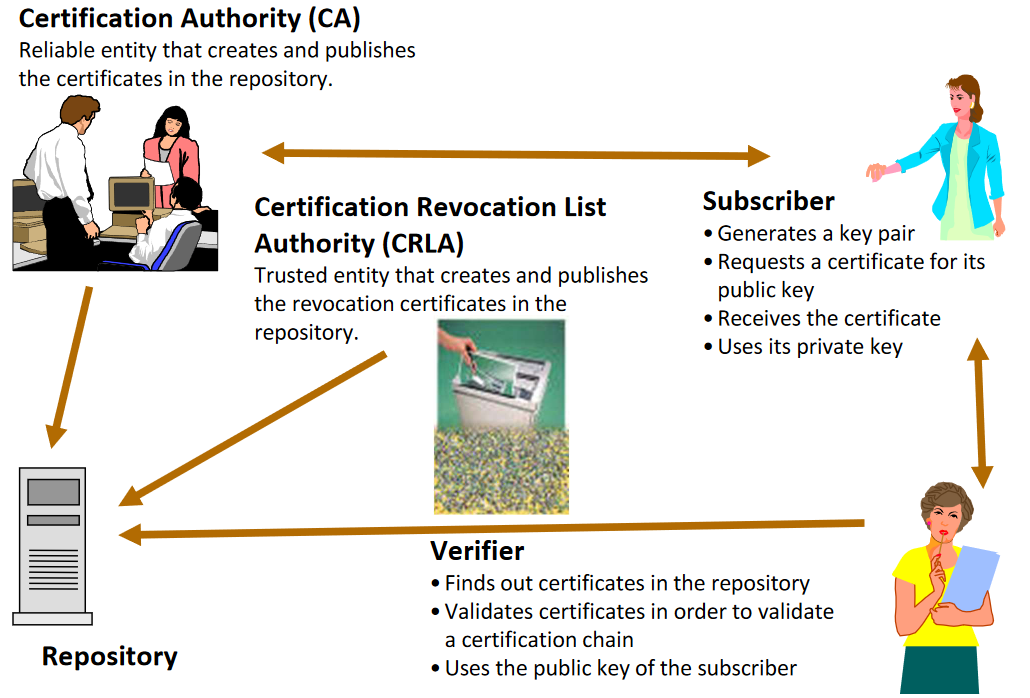
\includegraphics[scale=0.40]{23.png}
\end{figure}
A CA can establish trust relations by issuing public key certificates of other CAs or by requiring certification of its public key to other CAs. Some typical trust relations include:
\begin{itemize}
\item Flat: only the root CA is trusted. Verifying entities check the certificates validity with the public key of the CA.
\begin{figure}[H]
\centering
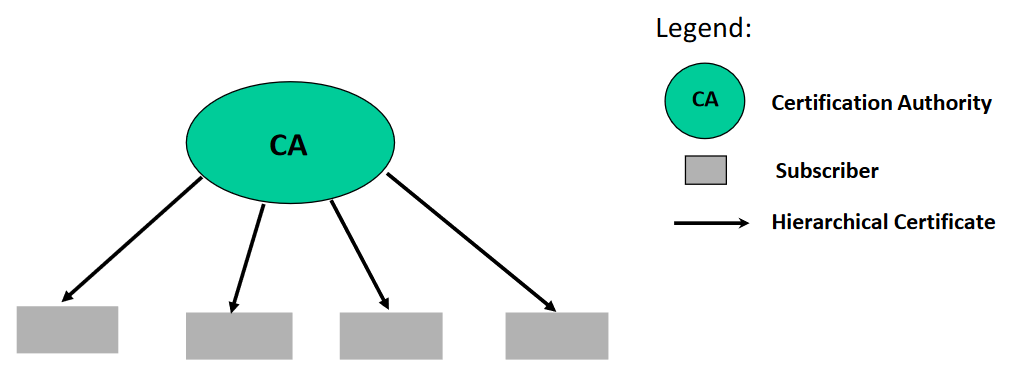
\includegraphics[scale=0.40]{24.png}
\end{figure}
\item Hierarchical: there is a tree of CAs. CAs issue certificates to subscribers and other CAs and verifying entities verify the certificates of the subscribers by
sequentially checking the certificates up to the root certificate (verifying entitites trust CA1)
\begin{figure}[H]
\centering
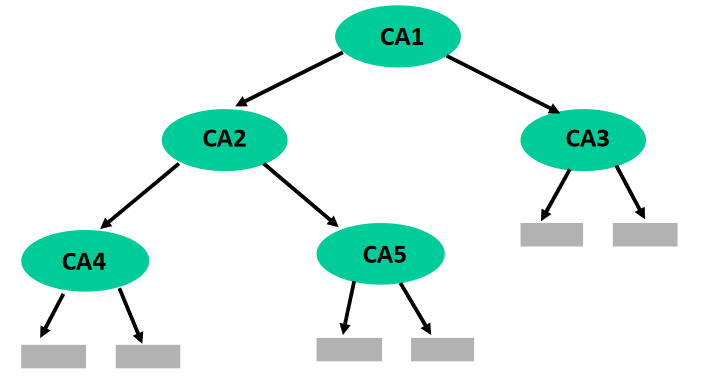
\includegraphics[scale=0.40]{25.png}
\end{figure}
The use of intermediary certificates protects the PKI root certificate and delegates the signing authority to another organization (better for scalability)
\item List of certificates: The verifying entities trust the keys of several root CAs. The verifying entities validate the chain of certificates that lead to any of the CAs
\begin{figure}[H]
\centering
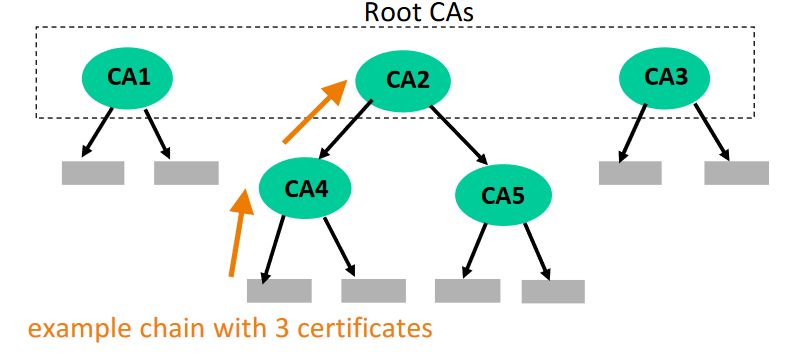
\includegraphics[scale=0.40]{26.png}
\end{figure}
\end{itemize}
Browsers and operating systems have root stores with lists of trusted CAs.
\subsubsection{Certificate Revocation}
A certificate may be withdrawn for several reasons:
\begin{itemize}
\item Corresponding private key compromised
\item Certificate owner does not operate service any longer
\item Key ownership has changed
\item ...
\end{itemize}
Two approaches may be used:
\begin{itemize}
\item Certificate revocation lists (CRL)
\begin{itemize}
\item Lists of revoked certificates
\item Should be regularly checked by the certificate holders
\item Intermediate certificates should be checked too
\item CRLs can become large
\end{itemize}
\item Online Certificate Status Protocol (OCSP)
\begin{itemize}
\item Allows live revocation checks over the network
\item Uses a request-response model
\item Information must be fresh
\item Servers must have high availability
\end{itemize}
\end{itemize}
There is also a method called OCSP stapling. The idea is that the web server obtains a fresh OCSP response and
"staples" it to the certificate given to the web browser. This is more efficient and secure, but not universally supported.

\section{Secret Key Management}
The management of secret keys deals with several aspects, such as key generation, distribution and lifetime.
\subsection{Key Generation}
Adequate random values generators should be used for appropriate key generation. Several sources of entropy may be used to create a random number:
\begin{itemize}
\item Ticks since boot
\item Current time
\item Low-level system info
\item ...
\end{itemize}
Key size depends on the algorithm's strength, lifetime and usage of the key, as well as the attacker's power.
\subsection{Key Distribution}
Perfect forward secrecy (PFS) is a desirable characteristic of a key agreement protocol. It gives assurance that session keys will not be compromised even if the private key of the server is compromised.\\
\\
PFS protects past sessions against future compromises of keys
\subsubsection{Manual Distribution}
Keys may be manually distributed through physical support. Usually done for personal or large sets of keys.
\subsubsection{Distribution With Shared Values}
Distribution with long-term shared secrets is useful, allowing the  exchanging temporary secrets between entities that already share some secret information. The exchange has the form:
$$
A \rightarrow B:\{K_s\}_{KEK}
$$
Where the secret key is encrypted using a symmetric cipher, with the $KEK$ key, only known by $A$ and $B$. $B$ verifies the message freshness and contents. This method does not assure PFS, as the disclosure of $KEK$  reveals all session keys that have been exchanged between the communicating parties.\\
\\
Instead of using a shared key, the receiver's public key may also be used.
\subsubsection{Distribution Without Shared Values}
The Diffie-Hellman algorithm is often used in scenarios with no shared values.\\
\\
In this algorithm, the objective is to obtain a secret number $K$, shared between $A$ and $B$, but without communicating it in clear.
\begin{itemize}
\item Choose two public prime numbers $m$ and $n$ ($n$ large).
\item $A$ generates a random number $x_a$ and calculates $y_a = m^{x_a} \mod n$.
\item $B$ generates a random number $x_b$ and calculates $y_b = m^{x_b} \mod n$.
\item $y_a$ and $y_b$ are made public.
\item Each party calculates $K$ locally:
$$
K = y_b^{x_a} \mod n = y_a^{x_b} \mod n
$$
\end{itemize}
This type of distribution does not provide authentication and is vulnerable to man-in-the-middle attacks. However, if both secret values a and b are ephemeral (e.g. used only once), then there is PFS.
\subsubsection{Distribution With Third Parties}
Distribution may be done through means of trusted third parties, such as a key distribution center. These centers act as mediators between the communicating parties, simplifying the management of long-term shared secrets.
\begin{figure}[H]
\centering
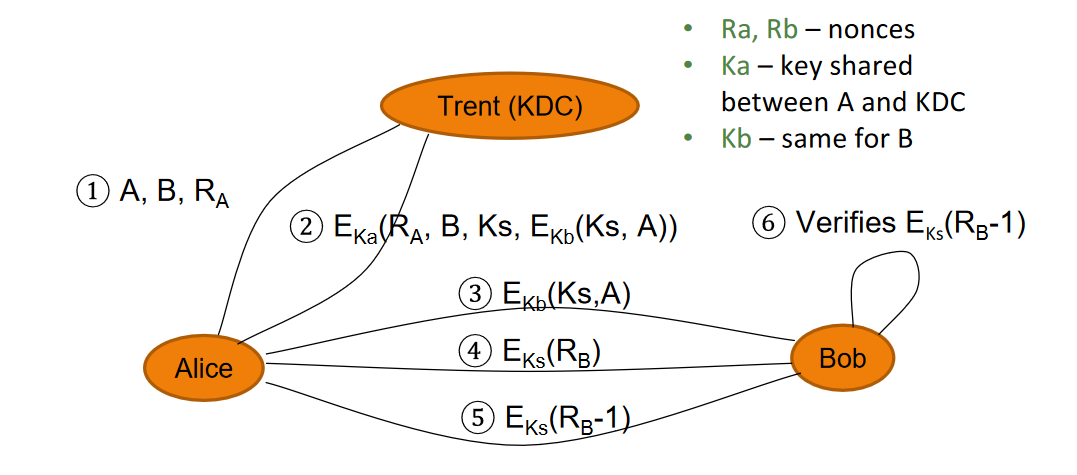
\includegraphics[scale=0.40]{27.png}
\end{figure}
This type of distribution assumes authentication and does not assure PFS.\\
\\
Kerberos is another frequently used algorithm. It uses a ticket granting service (TGT) that provides time-limited credentials (tickets) for several services/servers and an authentication service (AS), allowing clients to login.
\begin{figure}[H]
\centering
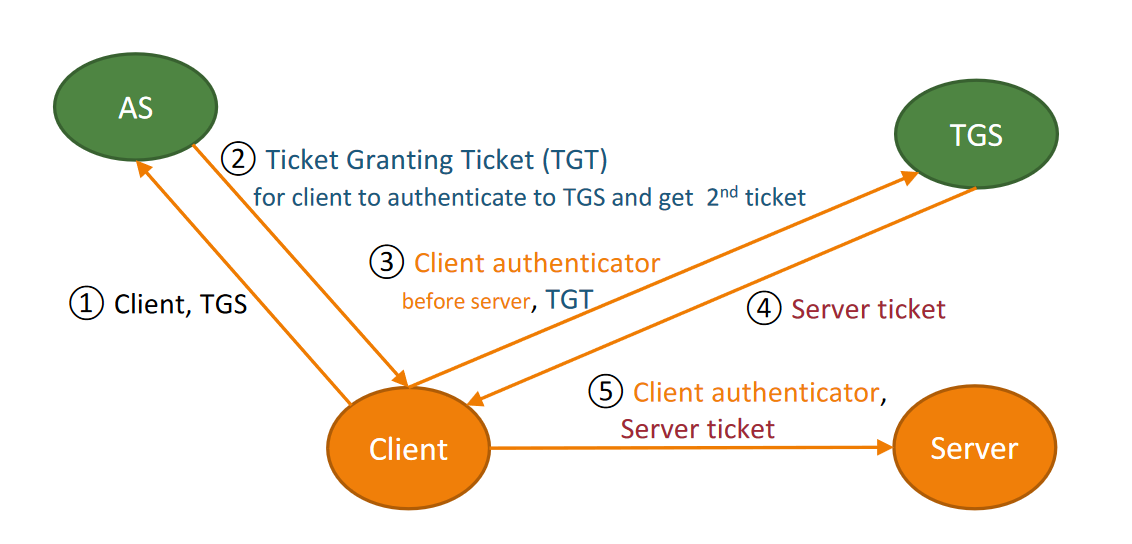
\includegraphics[scale=0.40]{28.png}
\end{figure}
Where tickets include client and server identifiers, timestamps with the beggining and end of validity and the session key value, all ciphered with the server key.\\
The authenticator has the client identifier and a timestamp of the request, ciphered with the session key.

\chapter{Networks}
\section{Network Models}
\subsection{OSI and Internet}
There are seven layers in the OSI model:
\begin{enumerate}
\item Physical
\item Data Link
\item Network
\item Transport
\item Session
\item Presentation
\item Application
\end{enumerate}
The network is not just computers and servers, there are also:
\begin{itemize}
\item Hubs: Send signals everywhere
\item Switches: Send frames only where they need to go
\item Routers: Look at the IP address from the incoming packet and forwards it. Have MAC address too.
\item Gateways: Access point to other networks, with possible change of addressing and networking technology.
\end{itemize}
\subsection{Address Resolution}
In layers 2 and 3, MAC and IP addresses are used, respectively. IP addresses identify the network and
the machine and MAC addresses may be converted to IPs with the ARP protocol. Some network ranges were reserved for private addressing.
\section{Network Vulnerabilities}
\subsection{Physical Layer}
\subsubsection{Hubs}
Hubs broadcast information on a shared medium, thus, are at threat of information leakage through sniffers.\\
\\
Anyone can connect to a hub even if it is physically secure.
\subsubsection{Sniffers}
Usually, network adapters operate in a non-promiscuous mode (only listen to what is sent to their MAC). Sniffers, on the other hand, read all frames, regardless of MAC.\\
\\
It is possible to indentify sniffers using tools (with several methods: latency, dns, os-specific, ...) or using the ARP method:
\begin{itemize}
\item Machines cache ARPs
\item Send a non-broadcast ARP with our correct MAC address
\item Then send a broadcast ping with the right IP but wrong MAC address
\item Only a machine which has our correct MAC address from the sniffed ARP will respond
\end{itemize}
To prevent sniffing, switches may be used instead of hubs (does not fully solve). It is also possible to prevent the effectiveness of sniffing by using one-time passwords and encryption.
\subsection{Data Link Layer}
Switches typically send frames only to the destination MAC address, and thus, reduce the sniffing problem. There are, however, some ARP vulnerabilities present:
\begin{itemize}
\item MAC flooding: attacker sends several unsolicited ARP messages, overwhelming the switch with entries. When the table is filled, some switches stop accepting connections and others revert to Hub mode
\item ARP Spoofing/Poisoning: An attacker sends a non-requested ARP message with a false IP-MAC address correspondence. ARP messages are in no way signed, so it is easy to falsify a message from any given MAC
\end{itemize}
Some preventive measures include the use of tools like $arpwatch$, to monitor the ARP to IP translation and the use of switches with fixed tables (with a cost in flexibility).
\subsection{Network Layer}
Routers support the indirect delivery of IP datagrams through the use of routing tables. Some threats in this layer include:
\begin{itemize}
\item Packet integrity: Data is not authenticated, so an attacker can change the source address of IP packets
\item Information lead and DoS: Users have little to no guarantee concerning the routing path taken by the packets. An attacker might corrupt the routing tables by sending routing-update messages and effectively hijack the route
\end{itemize}
\subsection{Transport Layer}
\subsubsection{UDP}
UDP  can be used to send and receive individual packets, without an established connection. It's just a thin addition to IP and is vulnerable to the same attacks.
\subsubsection{TCP}
TCP  can be used establish a connection to send and receive a data stream of bytes. An example of a TCP handshake:
\begin{figure}[H]
\centering
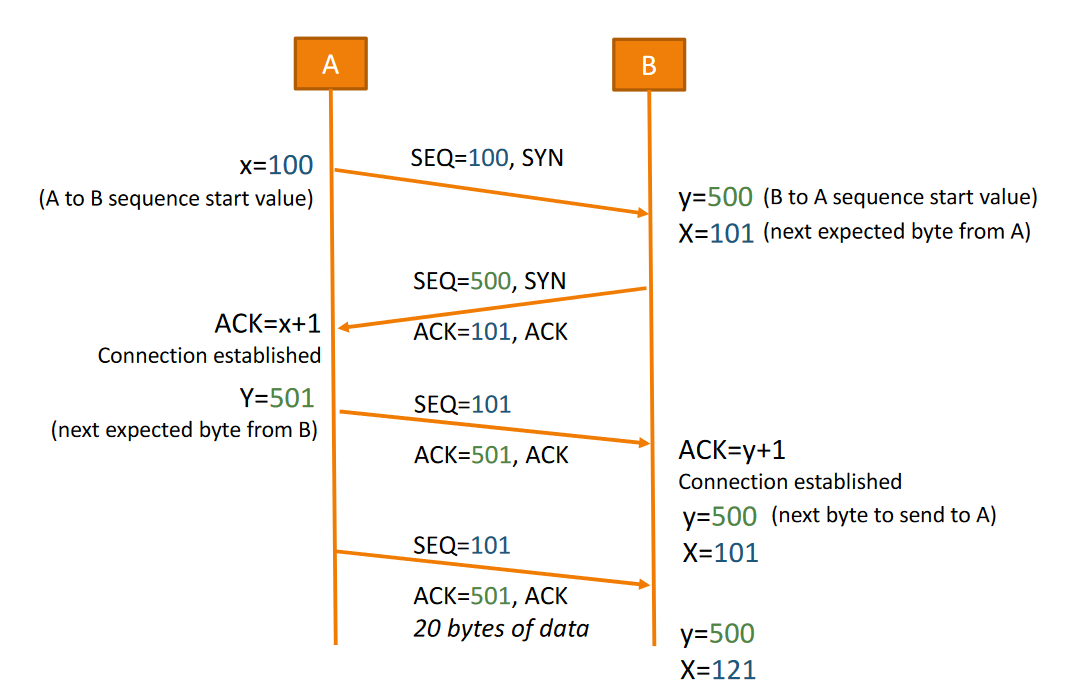
\includegraphics[scale=0.45]{9.png}
\end{figure}
There are different techniques for TCP hijecking, depending on the attacker’s capability to intercept communications:
\begin{itemize}
\item Full adversary-in-the-middle: the attacker is positioned to fully intercept the communication and  can intercept the sequence numbers and take over the connection. The tool $shijack$ is capable of doing this.
\begin{figure}[H]
\centering
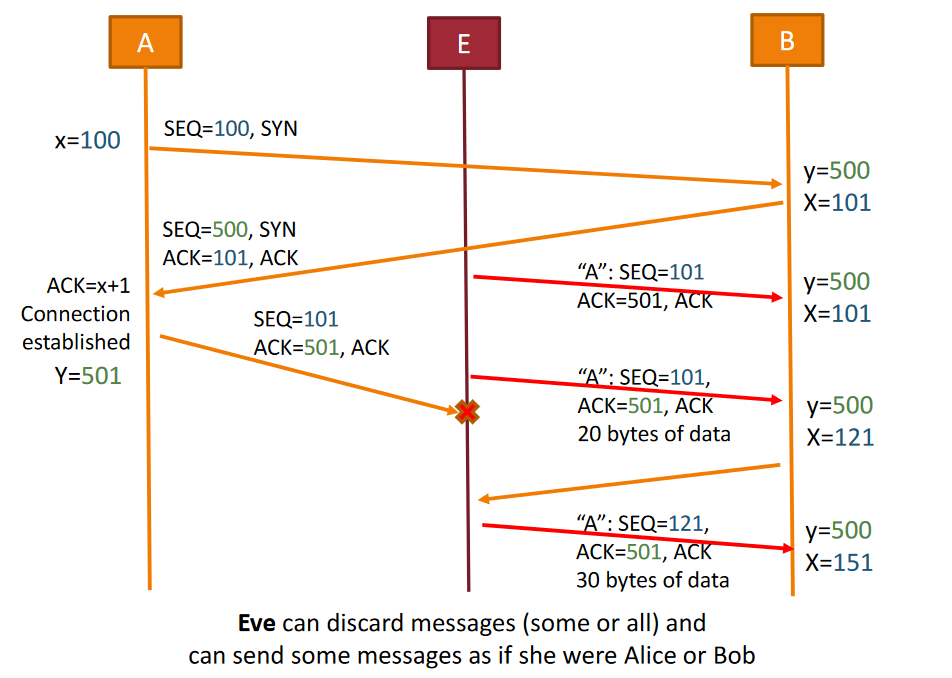
\includegraphics[scale=0.45]{10.png}
\end{figure}
\item Weak adversary-in-the-middle TCP hijack: the attacker can only eavesdrop and spoof packets (cannot drop packets). Attacker must now exploit de-synchronization between hosts. Once the sender and the receiver are desynchronized, only the attacker can create data segments with correct numbers
\begin{figure}[H]
\centering
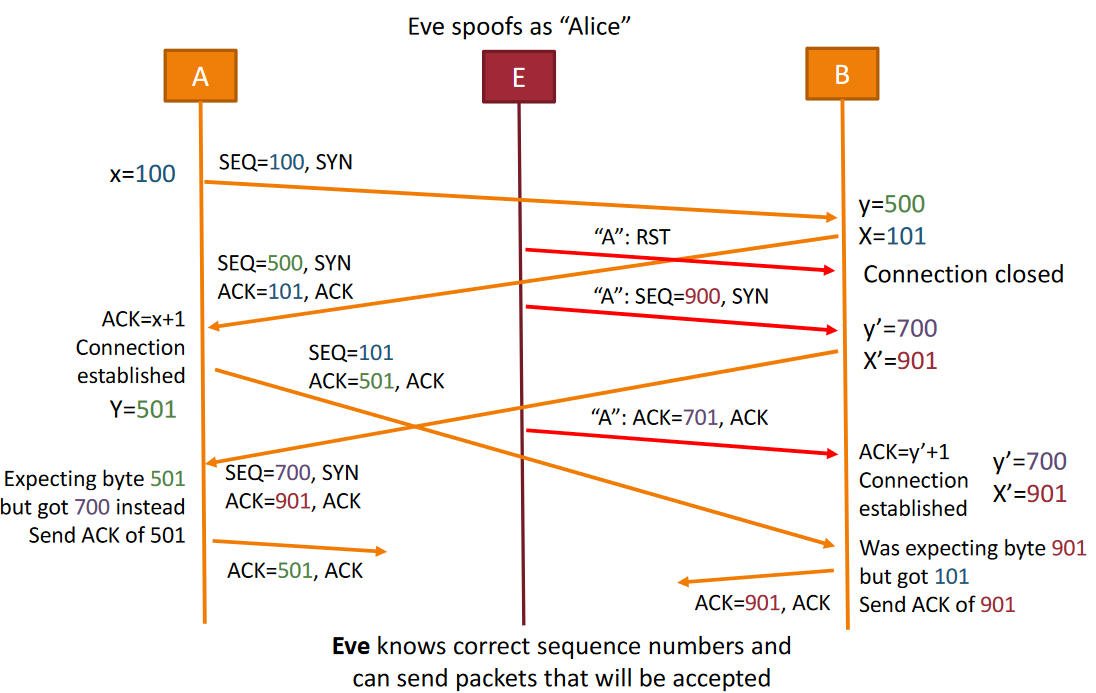
\includegraphics[scale=0.45]{11.png}
\end{figure}
The de-synchronization can be forged during the
creation of a TCP/IP connection with a reset and with false acknowledgements. It can also be done for an already established connection by sending blank data to displace sliding windows.
\item Blind TCP hijack: The attacker cannot capture return traffic from the host connection and only blindly sends malicious or manipulated packets. The attacker does not receive any confirmation of the desired effect through a packet capture and for  the attack to be successful, the attacker must guess the sequence numbers of the TCP packets
\end{itemize}
Another common TCP attacks is syn flooding. It consists of overloading a host with incomplete TCP/IP connection requests. There is no definite solution for IPv4 SYN flooding; SYN cookies may also be used to mitigate flooding:
\begin{figure}[H]
\centering
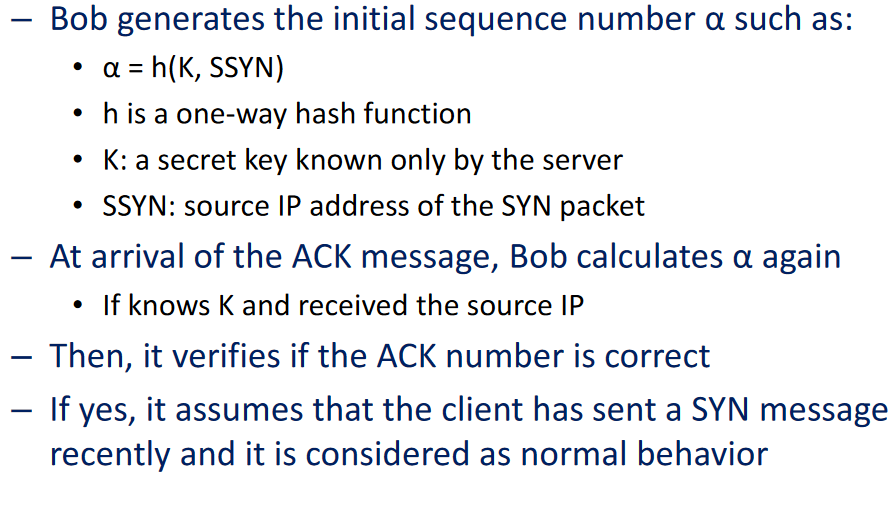
\includegraphics[scale=0.45]{12.png}
\end{figure}
Cooperation with firewalls and attack detectors is also helpful:
\begin{itemize}
\item Handshake relay: firewall stands in front of server and protects it until the handshake is complete
\item Gateway: firewall keeps the connection alive on server and terminates it if the client leaves the connection open but without traffic
\end{itemize}
\subsection{Application Layer}
\subsubsection{DNS}
DNS translates domain names to IP addresses. In 2008 the Kaminsky attack was found:
\begin{figure}[H]
\centering
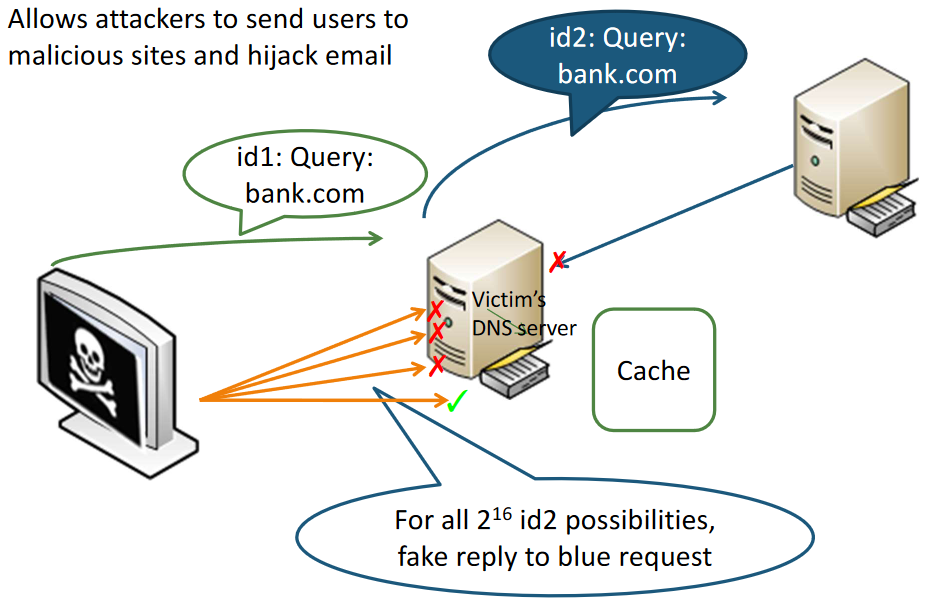
\includegraphics[scale=0.45]{13.png}
\end{figure}
The attack is successful if it can guess the query ID value.\\
\\
DNSSEC is DNS with digitally signed responses. Each zone has its own key-pair for signing and public Keys are published in the DNS itself. DNSSEC provides integrity and authenticity for RRs of the signed zones.
\subsubsection{RCE}
Remote code execution is a  class of software security vulnerabilities. Most programming languages have some way to generate code in runtime and execute it, which has the potential of being abused by a malicious actor.\\
\\
To prevent code injection, one must avoid using data as code as much as possible, as well as sanitize inputs.
\section{Network Security Models}
Gatekeeper for access control:
\begin{figure}[H]
\centering
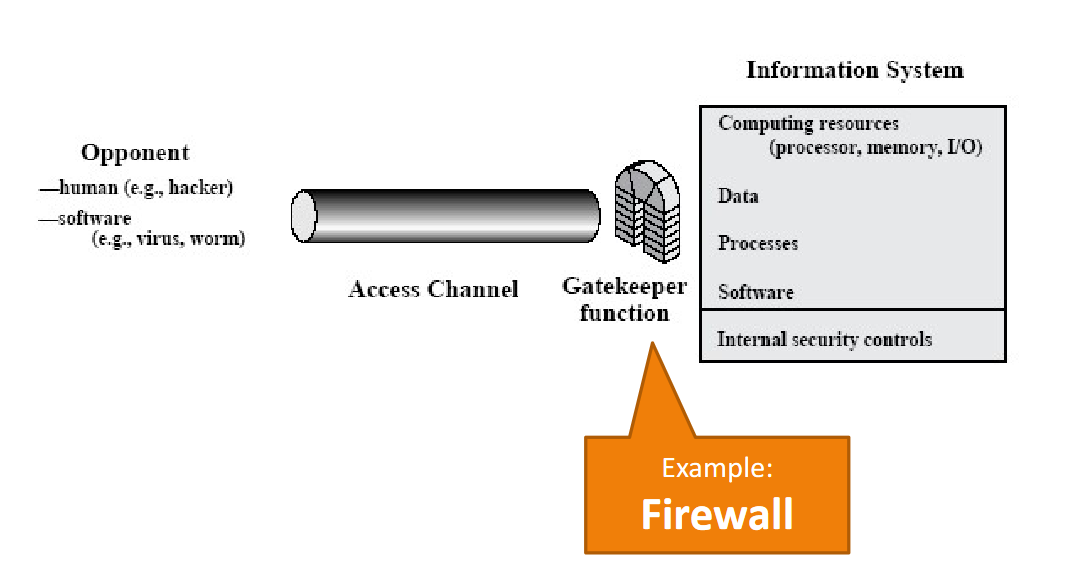
\includegraphics[scale=0.45]{14.png}
\end{figure}
Secure communication channel:
\begin{figure}[H]
\centering
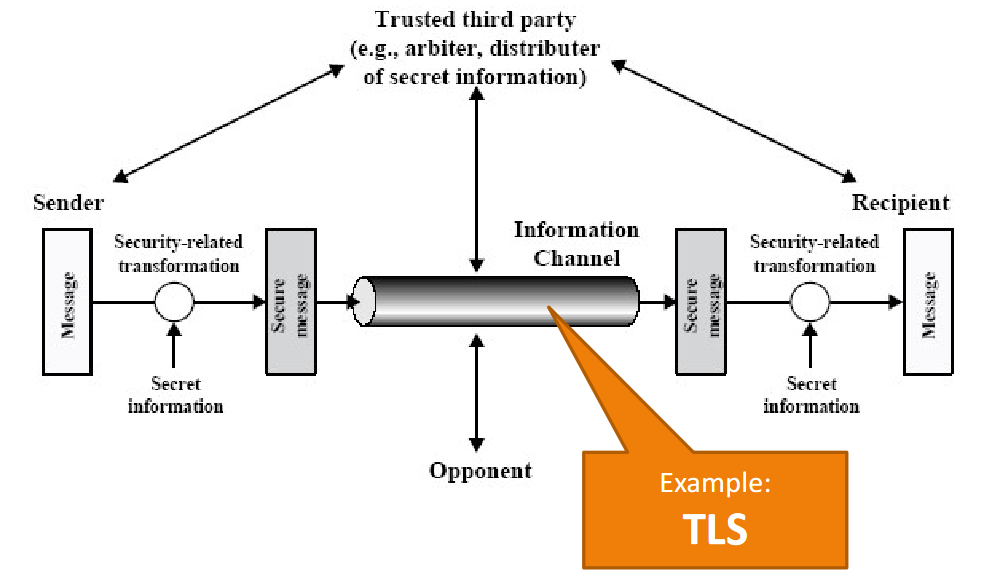
\includegraphics[scale=0.45]{15.png}
\end{figure}
\section{Firewalls and Intrusion Detection Systems}
A Firewall is a means of protecting a local system or network of systems from network threats, creating a perimeter of defense.\\
\\
Incoming TCP and UDP traffic should be denied by default and malformed packets should be blocked.
\subsection{Firewall Placement}
\subsubsection{Dual-Homed Host Firewall}
This architecture uses a bastion host with 2 home networks: IN and OUT
\begin{figure}[H]
\centering
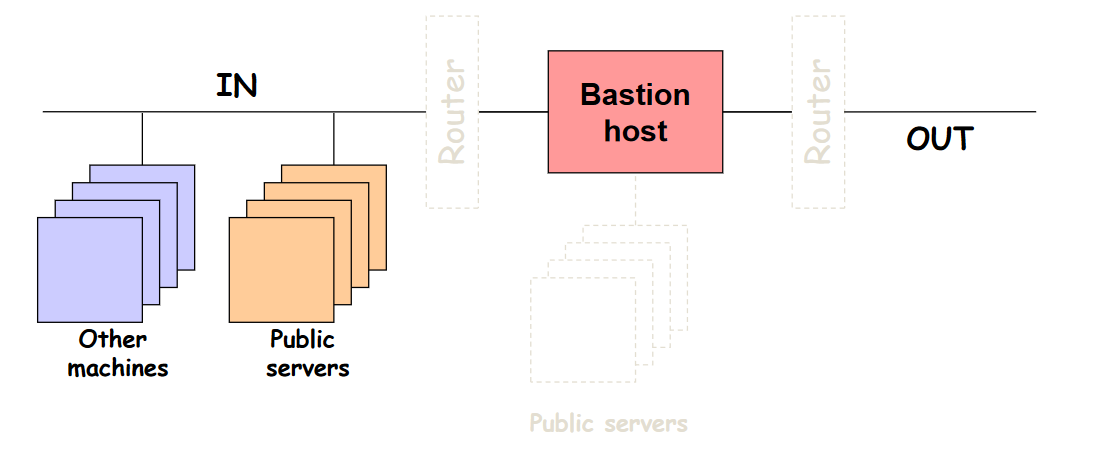
\includegraphics[scale=0.45]{16.png}
\end{figure}
It's a simple an resource-efficient topology, but has some disadvantages: compromising the machine deactivates the firewall, all the processing load is in a single machine, and public servers are within the protected network.
\subsubsection{Screened subnet}
This approach also has two internal subnets: IN and DMZ.
\begin{figure}[H]
\centering
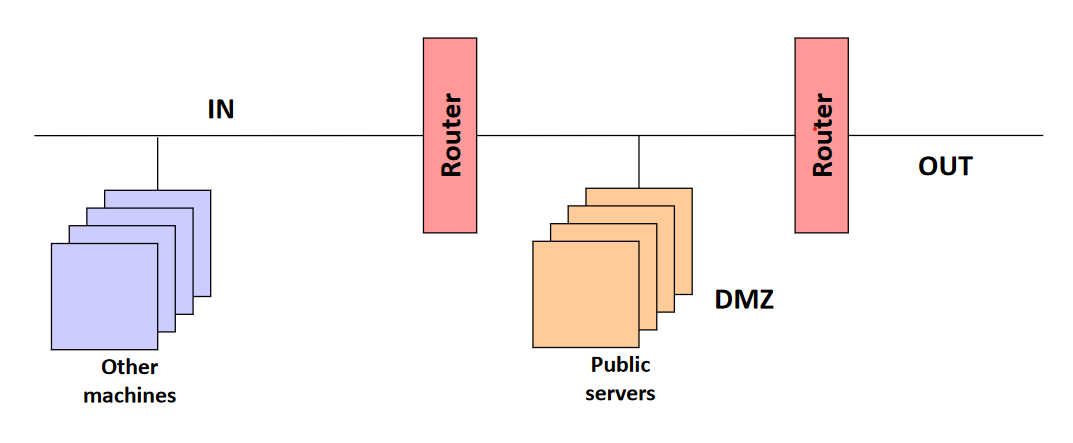
\includegraphics[scale=0.45]{17.png}
\end{figure}
There is a lower risk regarding the public services and of the firewall being compromised. However, there is also less control over the activities going on in the DMZ machines.
\subsection{Iptables}
Iptables has 3 chains (lists of rules): input, output forward. When a packet reaches a chain, the chain’s rules decide the packet’s fate: drop or accept.
\begin{figure}[H]
\centering
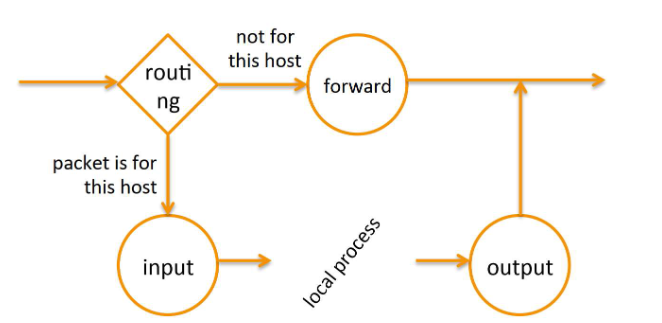
\includegraphics[scale=0.45]{18.png}
\end{figure}
\subsection{Types of Firewall}
There are several types of firewall:
\begin{itemize}
\item Packet filter:
\begin{itemize}
\item Reject packets depending on the IP and transport layer headers
\item Can be stateful or stateless
\end{itemize}
\item Circuit-level gateway:
\begin{itemize}
\item Control iterations at the transport layer (typically TCP "circuit")
\item Similar to application-level gateways
\end{itemize}
\item Application-level gateway:
\begin{itemize}
\item Control iterations at the application layer
\item Protocol-specific proxy
\end{itemize}
\end{itemize}
Packet filters are faster but harder to configure and are unable to protect against "misbehaving" protocols. On the other hand, application-level gateways are slower but easier to configure, allow for more authentication mechanisms and more fine-grained control, with the disadvantage of being less adaptable to new protocols.
\subsection{Intrusion Detection Systems}
An IDS is a software that has the function to detect, identify, and respond to unauthorized or abnormal activities in the targeted system. IDS' complement firewalls and are capable of:
\begin{itemize}
\item Deep packet inspection (look at packet contents)
\item Examine correlation among multiple packets
\end{itemize}
IDS' generate alarms and, as such, are prone to generate false positives/negatives.
\subsection{IDS classification}
There are several criteria to classify IDS:
\begin{figure}[H]
\centering
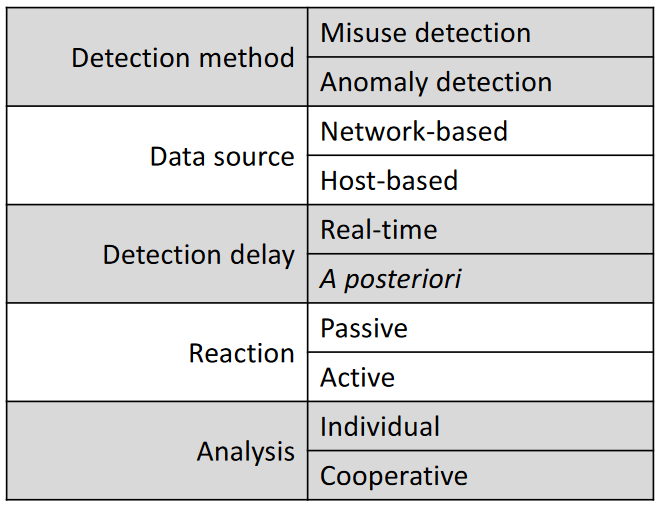
\includegraphics[scale=0.45]{19.png}
\end{figure}
\begin{itemize}
\item Detection method:
\begin{itemize}
\item Misuse detection: system activity analysis in search of known attack patterns (attack signatures)
\item Anomaly Detection: matches observed behavior with a model of normal behavior
\end{itemize}
\item Data source:
\begin{itemize}
\item  Network-Based IDS: capture and do traffic analysis on network data (e.g., packets)
\item Host-Based IDS: capture and do analysis on host data
\end{itemize}
\item Reaction:
\begin{itemize}
\item Passive: only detect and report the detection results
\item Active: respond to attacks
\end{itemize}
\end{itemize}

\section{SSH and TLS}
SSH is a secure communication application and
protocol over TCP. Allows secure remote sessions, file transfer and tunneling of traffic, while providing confidentiality and integrity.\\
\\
It has server authentication, being a trust-on-first-use model (vullnerable to man-in-the-middle). SSH also uses Diffie-Hellman for key exchange. User authentication may be done through a password or a signature with the client's private key.
\subsection{SSH Tunneling}
In the client machine, a mapping is created between a local TCP port and a port in the remote machine. The client application is configured to use the local port and, when using it, it will securely interact via SSH.\\
\\
Tunneling is transparent for apps, but complex for admins and provides low flexibility for devs and users.
\subsection{TLS}
TLS provides secure channels over TCP/IP, authentication, integrity, confidentiality, and key distribution.
\begin{itemize}
\item Handshake:
\begin{itemize}
\item Alice and Bob use their certificates, private keys to authenticate each other and exchange a shared secret
\end{itemize}
\item Key derivation: 
\begin{itemize}
\item Alice and Bob use shared secret to derive set of keys
\end{itemize}
\item Data transfer:
\begin{itemize}
\item Data to be transferred is broken up into series of records
\item Data records: the stream is broken into a series of records, each with its length and MAC
\item Sequence numbers are used to prevent replay attacks and the order of records
\item Record types are used to prevent truncation (early closure) attacks. Type 0 is for data and type 1 is for closure
\end{itemize}
\end{itemize}
\begin{figure}[H]
\centering
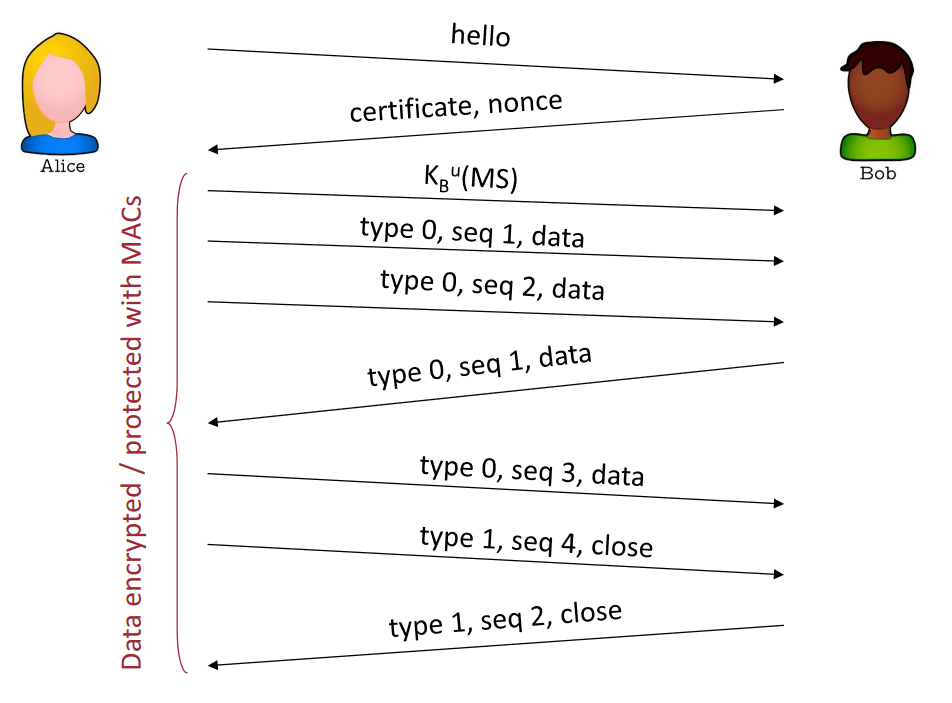
\includegraphics[scale=0.40]{20.png}
\end{figure}
\subsection{TLS Protocols}
There are two TLS protocols:
\begin{itemize}
\item Record protocol: creation and verification of secure messages
\item Handshake Protocol: exchange of identity and supported cipher suites, authentication of the communicating parties and key distribution
\end{itemize}
The record protocol can be described as follows:
\begin{figure}[H]
\centering
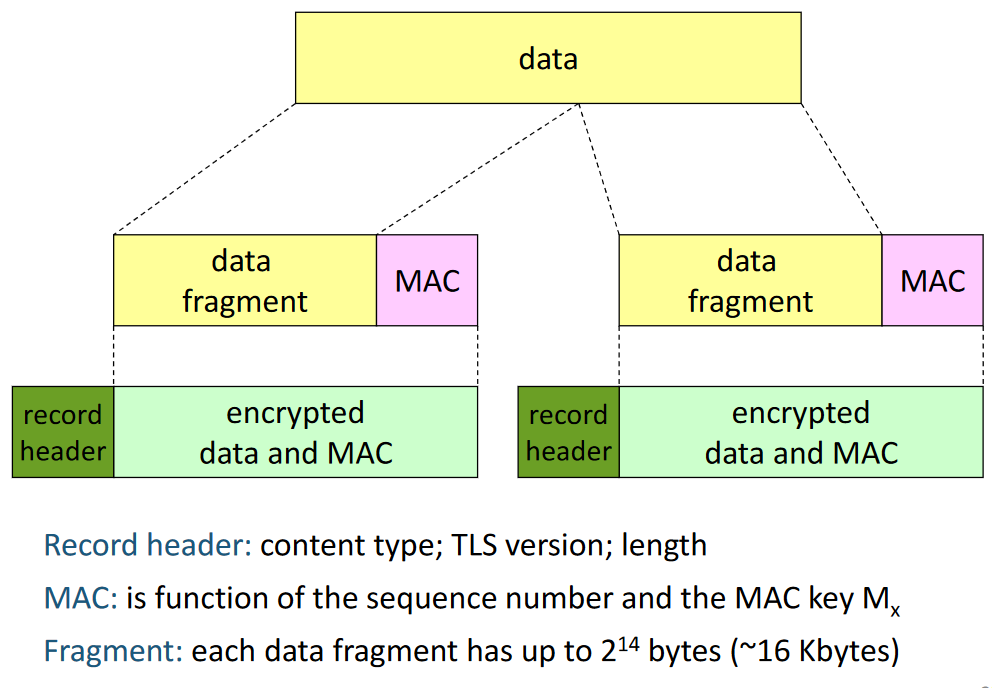
\includegraphics[scale=0.40]{21.png}
\end{figure}
And the handshake is as follows:
\begin{figure}[H]
\centering
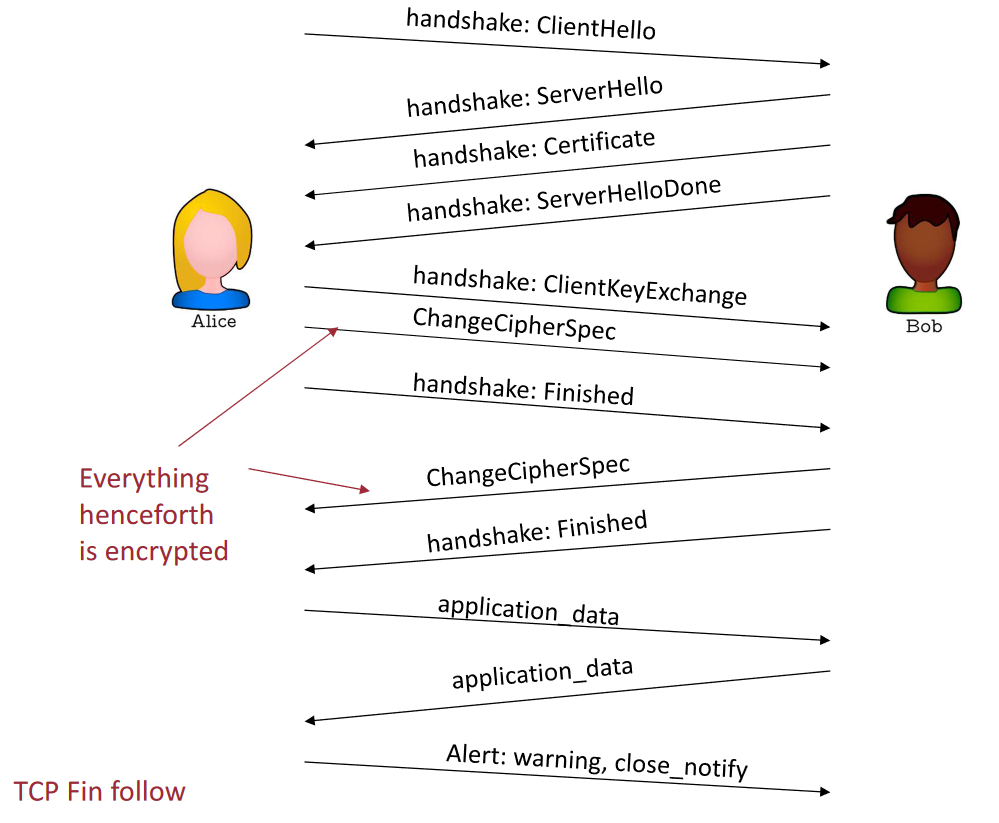
\includegraphics[scale=0.40]{22.png}
\end{figure}
\subsection{Key Derivation}
The client nonce, server nonce, and pre-master secret input into pseudo random-number generator, produce a master secret.\\
\\
Master secret and nonces input into another pseudo
random-number generator, produce key block, cut into several other keys, such as the server and client MAC and encryption keys and initialization vectors.
\section{Authentication}
Authentication services must handle problems of security and trustworthyness. Their end goal is one of entity (user, machine, service) authentication, facilitating protocol usage and preventing impersonation from attackers.
\subsection{Authentication With Passwords}
This type of authentication requires the user to memorize a password and provide it when prompted. It is simple but passwords may be poorly selected by users, making them susceptible to password attacks.\\
\\
A key derivation function (KDF), such as hashing, is often used when storing passwords in order to prevent their hijacking by attackers. A modern password-based KDF is PBKDF2, which uses a cryptographic hash function, salt and a high iteration count.
\subsubsection{One-Time Passwords (OTP)}
This variation requires the validation of a one-time password regarding a secret stored for the user. Such a password is only valid once and thus, pointless for an attacker to capture.\\
\\
Has better security  in remote authentications over insecure networks or in insecure terminals, however, some implementations may require the users to use some device/application to generate the one-time passwords.
\subsubsection{Challenge-Response}
This method requires the authenticator to provide a challenge and the user being authenticated transforms the challenge using the secret that he shares with the authenticator.\\
\\
Its secure for authentication over unsecure networks, but the authenticator needs to have shared secrets with all users.
\subsection{Biometric Authentication}
The user is validated through biometrical data: fingerprint, physiognomy,... It solves the problem of choosing a good password and does not rely on the user's memory, but can be deceived sometimes and does not  allow the transference of authentication between subjects.\\
\\
The principle of biometric authentication has two phases:
\begin{itemize}
\item Registration: acquisition of information about the person
\item Authentication: checking the obtained biometric data with the stored template
\end{itemize}
It should fulfill the following desirable properties: universality, unicity, stability, correctness, convenience and acceptance.
\subsection{Authentication Protocols}
\subsubsection{Password Protocols}
There is PAP and CHAP, both protocols are used by PPP (Point-to-Point Protocol). Authentication is unidirectional ($A$ authenticates $U$)
\begin{itemize}
\item PAP: simple exchange of pair UID/password. Insecure, as the password is sent in plain text:
\begin{align}
&U \rightarrow A: username,\; password\\
&A \rightarrow U: OK/not \; OK
\end{align}
\item Challenge Handshake Authentication Protocol (CHAP): 
\begin{align}
&U \rightarrow A: username\\
&A \rightarrow U: authID, \; challenge\\
&U \rightarrow A: Hash(authID,\; passoword,\; challenge)\\
&A \rightarrow U: OK/not \; OK
\end{align}
In this version, $A$ stores the passwords, however, that problem may be solved by using only a hash of the password.
\end{itemize}
\subsubsection{One-Time Password Protocols}
\begin{itemize}
\item S/Key: Authenticator gives user a sequence of one-time passwords
$$
OPT_1 = Hash(seed,password) \; ... \; OPT_n = Hash(OTP_{n-1})
$$
For each user, the authenticator stores only the seed of the one-time password sequence and the current index. The authentication process is as follows:
\begin{itemize}
\item Authenticator sends index to the user
\item User sends $P = OPT_{index-1}$ to the authenticator (the one-time password)
\item Authenticator computes $Hash(P)$ and compares with stored $OPT_{index}$
\item If values are equal, then success, server stores $index-1$ and $OPT_{index-1}$
\item On the first time, the authenticator sends $index = n$, next $index = n-1$, etc.
\end{itemize}
\item RSA SecurID: generates a unique number every minute, essentially OPTs. The authentication process is as follows:
\begin{itemize}
\item The user generates a one-time password, combining a PIN with the card number
\item The RSA server performs the same operation and verifies if the values are equal
\item Server is synchronized with real time (RSA Security Time Synchronization)
\end{itemize}
\end{itemize}
\subsubsection{Asymmetric Keys Protocols}
The main protocol used with asymmetric keys is EKE. It does a password-authenticated key agreement and is resistant to dictionary attacks.
\begin{figure}[H]
\makebox[\textwidth][c]{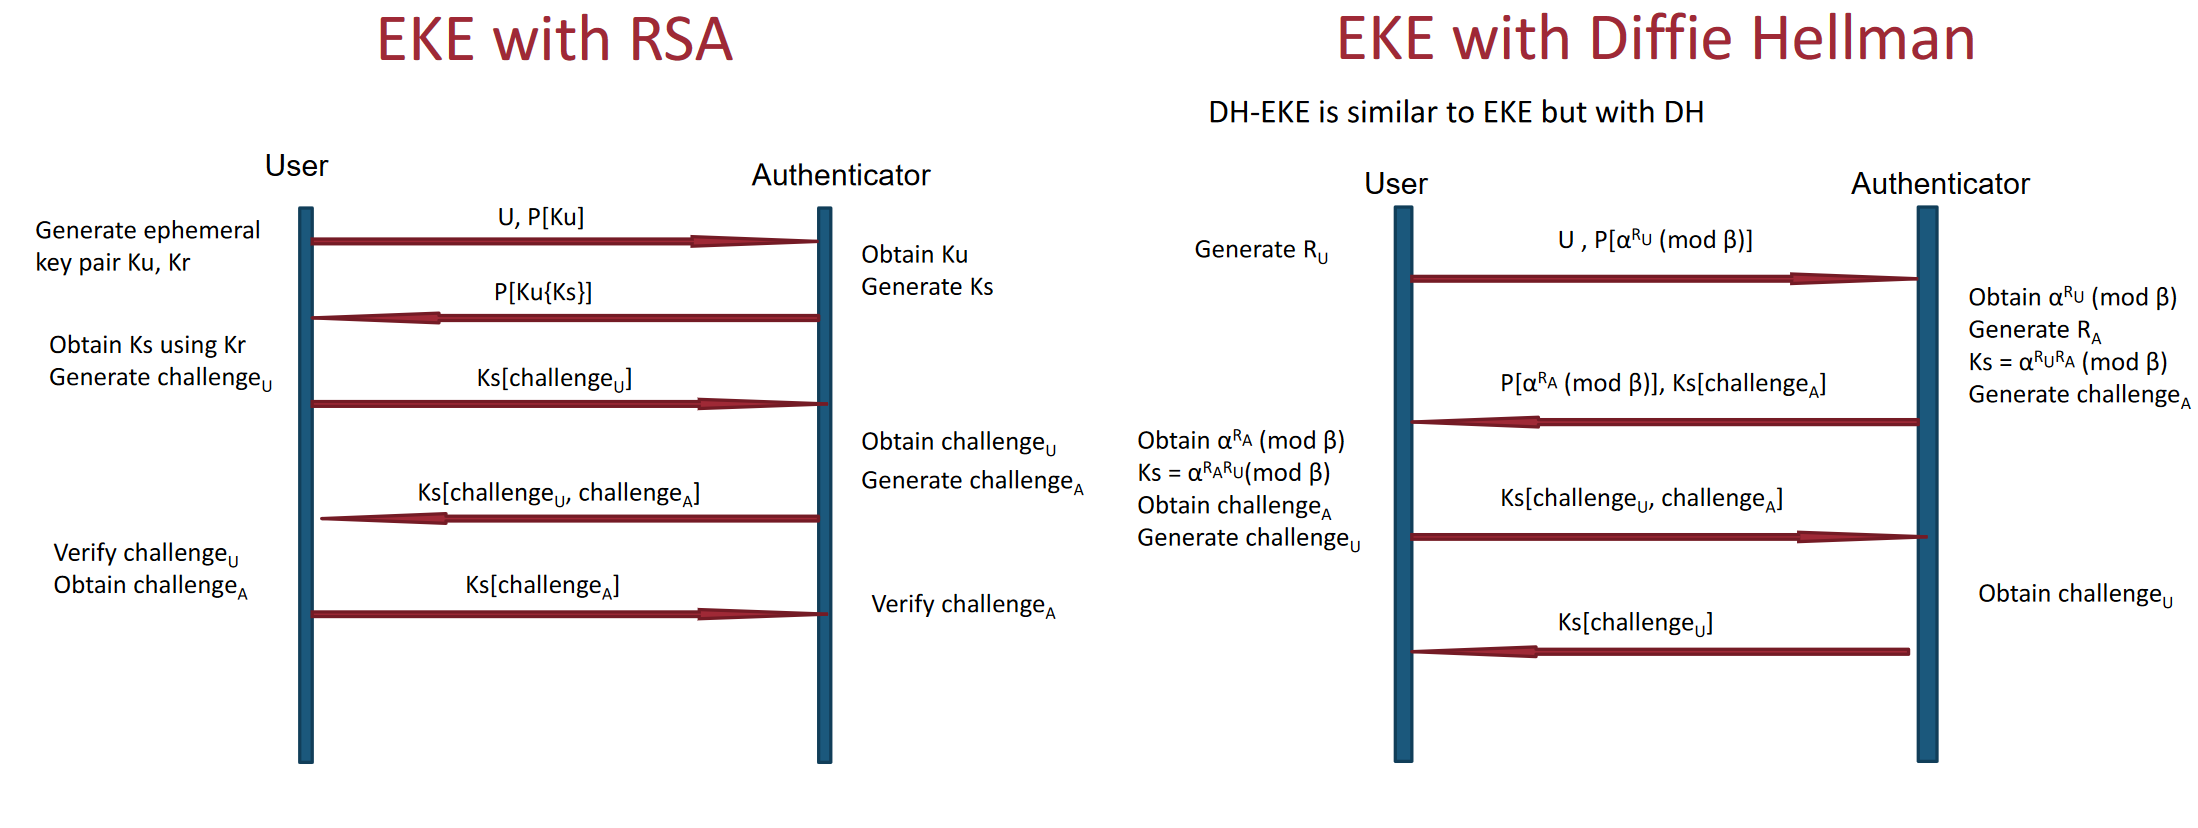
\includegraphics[scale=0.35]{29.png}}
\end{figure}
It's safe from dictionary attacks since, even if an attacker was successful decrypting the public key, it would still have to compute the private key to obtain the the session key (i.e. decrypt $K_u\{K_s\}$).\\
\\
It is also protected against man-in-the-middle and replay attacks. However, an attack to the password database in the authenticator would give access to $P$. The solution consists in only storing $Hash(P) = \pi$:
\begin{figure}[H]
\centering
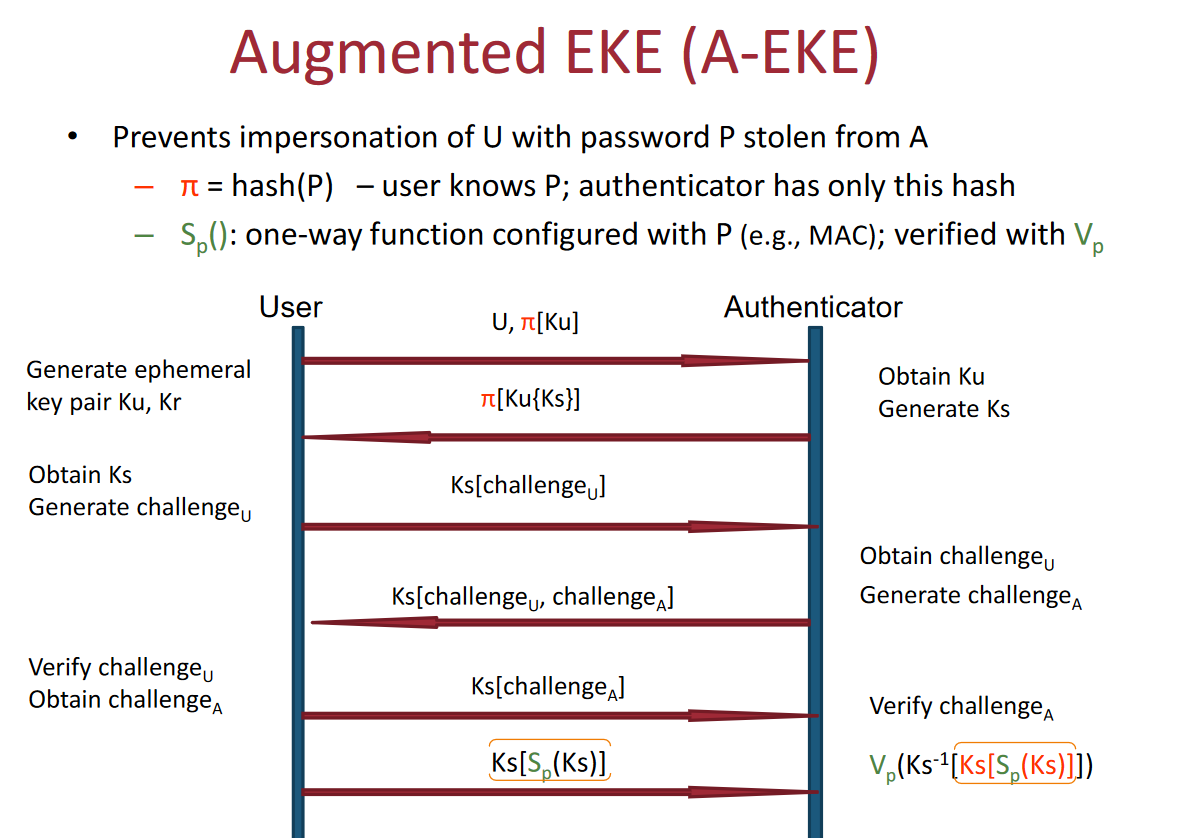
\includegraphics[scale=0.4]{30.png}
\end{figure}
The $Sp$ function could be, for example, a  cryptographic hash function combined with a unique salt for each user and the $Vp$ function could be a time-constant comparison to mitigate timing attacks.
\subsubsection{Web Authentication Protocols}
\begin{itemize}
\item HTTP Basic authentication: when user asks for protected page, browser asks user for username and password for that page and sends them encoded in Base64
\item HTTP Digest authentication: server sends a similar digest or nonce, the browser sends a hash instead of credentials
\item In HTTPS, SSL and TLS are used
\item FIDO2 user authentication: based on user-controlled cryptographic authenticators, such as a smartphone or hardware security key
\item Session-based authentication: server sends cookie with session identified to the client. Whenever browser sends request to the server, cookie is inserted automatically
\end{itemize}
\subsubsection{Web Single-Sign On Protocols}
Single-sign on was developed as a solution for users who need to authenticate themselves in many devices, managing several passwords.\\
\\
OpenID is the main single-sign on protocol. When a user wants to login in a relying party (OpenID supporter), the following exchange occours:
\begin{figure}[H]
\centering
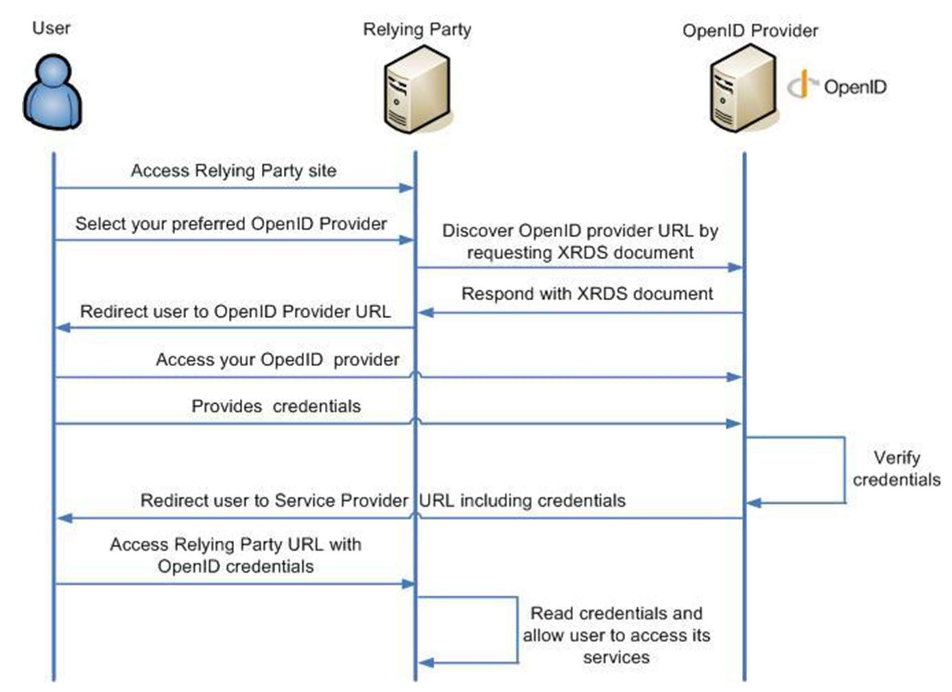
\includegraphics[scale=0.4]{31.png}
\end{figure}
\end{document}

%next: 7c